\chapter{Vibrations of a viscoelastic bar}
\label{chapter:viscoelastic-bar-vibrations}

Consider the elastic bar shown in figure~\ref{fig:viscoelastic-bar}. It is fixed on the left hand side and free on the right, has a length of $L$ and can undergo longitudinal motion as described by the function $u(x,\,t)$. We want to calculate its (undamped) natural frequencies $\omega_0$ and associated damping ratios $\zeta$.

\begin{figure}[h]
\centering
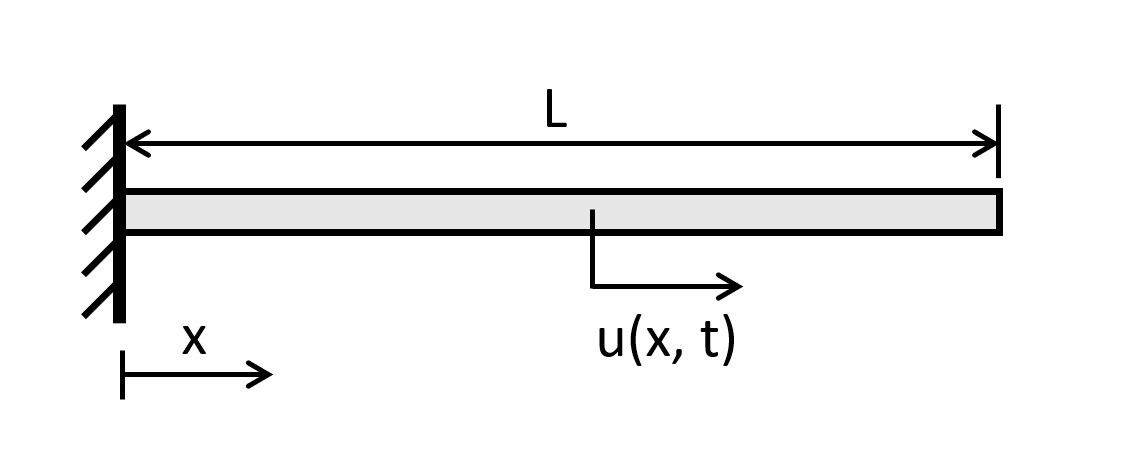
\includegraphics[width=0.5\textwidth]{figures/appendix/viscoelastic-bar}
\caption{Kinematics and boundary conditions of the bar}
\label{fig:viscoelastic-bar}
\end{figure}

The material of the bar is assumed to behave according to the viscoelastic Kelvin-Voigt model, which expresses the stress $\sigma$ in the bar as
%
\begin{equation}
\sigma = E\,\varepsilon + \eta\,\dot{\varepsilon}\label{eq:viscoelastic-bar-material}
\end{equation}

where $\varepsilon = \frac{\partial\,u}{\partial\,x}$ is the longitudinal strain, $E$ the elastic modulus and $\eta$ the viscosity of the material. The acceleration at every point in the bar is given by \textcolor{red}{Source?}
%
\begin{equation}
\rho\,\frac{\partial^2\,u}{\partial\,t^2} = \frac{\partial\,\sigma}{\partial\,x}\label{eq:viscoelastic-bar-kinetic}
\end{equation}

where $\rho$ is the bar's density. Combining the equations (\ref{eq:viscoelastic-bar-material}) and (\ref{eq:viscoelastic-bar-kinetic}) and multiplying with the cross section area $A$ results in the equation of motion
%
\begin{equation}
\rho A\,\frac{\partial^2\,u}{\partial\,t^2} = EA\,\frac{\partial^2\,u}{\partial\,x^2} + \eta A\,\frac{\partial^3\,u}{\partial\,x^2\,\partial\,t}.\label{eq:viscoelastic-bar-motion}
\end{equation}

This partial differential equation can be solved by separation of variables. The solution is assumed as $u(x,\,t) = X(x)\,T(t)$, a product of two functions depending on $x$ and $t$ respectively. Inserting this into the equation of motion (\ref{eq:viscoelastic-bar-motion}) and separating terms depending on $x$ from terms depending on $t$ leads to
%
\begin{align}
\rho A\,X(x)\,\ddot{T}(t) &= EA\,X''(x)\,T(t) + \eta A\,X''(x)\,\dot{T}(t)\notag \\
\frac{X''(x)}{X(x)} &= \frac{\ddot{T}(t)}{\frac{EA}{\rho A}\,T(t) + \frac{\eta A}{\rho A}\,\dot{T}(t)} =: -\frac{\rho A}{EA}\,\omega_0^2\label{eq:viscoelastic-bar-separated}
\end{align}

Apply the usual argument: As one side of the equation depends on position and the other on time they have to be constant in order to be equal. We choose that constant to be $-\frac{\rho A}{EA}\,\omega_0^2$ and obtain the two ordinary differential equations
%
\begin{align}
\ddot{T}(t) + \frac{\eta A}{EA}\,\omega_0^2\,\dot{T}(t) + \omega_0^2\,T(t) = 0,\label{eq:viscoelastic-bar-t} \\
X''(x) + \frac{\rho A}{EA}\,\omega_0^2\,X(x) = 0.\label{eq:viscoelastic-bar-x}
\end{align}

The time equation (\ref{eq:viscoelastic-bar-t}) describes a damped harmonic oscillator with undamped natural frequency $\omega_0$ and damping ratio
%
\begin{equation}
\zeta = \frac{1}{2}\,\frac{\eta\,A}{EA}\,\omega_0\label{eq:viscoelastic-bar-result-zeta}
\end{equation}

as determined by the coefficients of the equation. The last remaining task is to determine the natural frequencies $\omega_0$ which solve the second differential equation (\ref{eq:viscoelastic-bar-x}) while also satisfying the boundary conditions of the bar. The general solution of (\ref{eq:viscoelastic-bar-x}) is
%
\begin{equation}
X(x) = C\cdot\sin\left(\sqrt{\frac{\rho A}{EA}}\,\omega_0\,x - \varphi\right).
\end{equation}

Boundary condition on the fixed end:
%
\begin{align}
u(0,\,t) = 0: \quad\quad\quad X(0)\,T(t) &= 0 \notag \\
C\cdot\sin(-\varphi) &= 0 \notag \\
\varphi &= 0
\end{align}

The case $T(t) = 0$ was ignored here because it is of no interest. The boundary condition for the free end is
%
\begin{align}
\sigma(L,\,t) = 0: \quad\quad E\,\varepsilon(L,\,t) + \eta\,\dot{\varepsilon}(L,\,t) &= 0 \notag \\
EA\,\frac{\partial u}{\partial x}(L,\,t) + \eta A\,\frac{\partial^2 u}{\partial x\,\partial t}(L,\,t) &= 0 \notag \\
EA\,X'(L)\,T(t) + \eta A\,X'(L)\,\dot{T}(t) &= 0 \notag \\
(EA\,T(t) + \eta A\,\dot{T}(t))\,X'(L) &= 0 \notag \\
\ddot{T}(t)\,X'(L) &= 0 \notag
\end{align}

And therefore the solution for the natural frequencies is
%
\begin{align}
X'(L) &= C\cdot\sqrt{\frac{\rho A}{EA}}\,\omega_0\cos\left(\sqrt{\frac{\rho A}{EA}}\,\omega_0\,L\right) = 0, \notag \\
\omega_0 &= \frac{\pi(2k - 1)}{2L}\cdot\sqrt{\frac{EA}{\rho A}},\quad k \in \mathbb{Z}.\label{eq:viscoelastic-bar-result-omega}
\end{align}

And finally, with equations (\ref{eq:viscoelastic-bar-result-zeta}) and (\ref{eq:viscoelastic-bar-result-omega}) the damping ratio follow as
%
\begin{equation}
\zeta = \frac{\pi(2k - 1)}{4L}\cdot\frac{\eta A}{\sqrt{\rho A \cdot EA}},\quad k \in \mathbb{Z}.
\end{equation}

\chapter{Cubic Spline Interpolation}

Cubic splines are used to define some of the geometric features of the bow, namely the profile curve, width and layer heights.

\section{Cubic $C^2$ Spline}

Consider $n$ points $(x_{0},\,y_{0}) \ldots (x_{n-1},\,y_{n-1})$ with increasing values of $x$.
We define the differences $\Delta x_{i} = x_{i+1} - x_{i}$ and $\Delta y_{i} = y_{i+1} - y_{i}$ as well as the slope $\delta_{i} = \Delta y_{i} / \Delta x_{i}$ of the secant line between two successive points.

For each interval $x \in [x_{i},\,x_{i+1}]$ the data is interpolated by the cubic polynomial
%
\begin{align}
f_{i}(x) &= h_{00}(t)\,y_{i} + h_{10}(t)\Delta x_{i}\,m_{i} + h_{01}(t)\,y_{i+1} + h_{11}(t)\Delta x_{i}\,m_{i+1} \\
f_{i}'(x) &= \frac{h_{00}'(t)}{\Delta x_{i}}\,y_{i} + h_{10}'(t)\,m_{i} + \frac{h_{01}'(t)}{\Delta x_{i}}\,y_{i+1} + h_{11}'(t)\,m_{i+1} \\
f_{i}''(x) &= \frac{h_{00}''(t)}{\Delta x_{i}^2}\,y_{i} + \frac{h_{10}''(t)}{\Delta x_{i}}\,m_{i} + \frac{h_{01}''(t)}{\Delta x_{i}^2}\,y_{i+1} + \frac{h_{11}''(t)}{\Delta x_{i}}\,m_{i+1}
\end{align}
%
where $y_{i}$, $y_{i+1}$ and $m_{i}$, $m_{i+1}$ are the values and slopes at the interval boundaries, respectively and $h_{00}(t)\,\ldots\,h_{11}(t)$ are the hermite basis functions, defined as
%
\begin{equation}
\begin{aligned}
h_{00}(t) &= 2\,t^3 - 3\,t^2 + 1 \\
h_{10}(t) &= t^3 - 2\,t^2 + t \\
h_{01}(t) &= -2\,t^3 + 3\,t^2 \\
h_{11}(t) &= t^3 - t^2
\end{aligned}
\quad
\begin{aligned}
h_{00}'(t) &= 6\,t^2 - 6\,t \\
h_{10}'(t) &= 3\,t^2 - 4\,t + 1 \\
h_{01}'(t) &= -6\,t^2 + 6\,t \\
h_{11}'(t) &= 3\,t^2 - 2\,t
\end{aligned}
\quad
\begin{aligned}
h_{00}''(t) &= 12\,t - 6 \\
h_{10}''(t) &= 6\,t - 4 \\
h_{01}''(t) &= -12\,t + 6 \\
h_{11}''(t) &= 6\,t - 2
\end{aligned}
\end{equation}
%
with $t = (x - x_{i})/(x_{i+1} - x_{i})$. The resulting spline by definition already interpolates the given function values and is $C^1$ continuous since adjacent segments share the same value and slope at the interval boundaries.
To determine the $n$ unknown slopes $m_{i}$ we require the second derivatives at the connection points to match as well, making the curve $C^2$ continuous. This gives us $n-2$ continuity conditions, leaving two more conditions to make the problem uniquely determined.
Those additional conditions are obtained from boundary considerations, e.g. by specifying the spline's first and/or second derivatives at the left and right endpoints.

%https://math.stackexchange.com/questions/62360/natural-cubic-splines-vs-piecewise-hermite-splines

Continuity conditions $f_{i-1}''(x_{i}) = f_{i}''(x_{i})$ for $i = 1 \ldots n-2$:
%
\begin{align}
&\frac{h_{00}''(1)}{\Delta x_{i-1}^2}\,y_{i-1} + \frac{h_{10}''(1)}{\Delta x_{i-1}}\,m_{i-1} + \frac{h_{01}''(1)}{\Delta x_{i-1}^2}\,y_{i} + \frac{h_{11}''(1)}{\Delta x_{i-1}}\,m_{i} = \frac{h_{00}''(0)}{\Delta x_{i}^2}\,y_{i} + \frac{h_{10}''(0)}{\Delta x_{i}}\,m_{i} + \frac{h_{01}''(0)}{\Delta x_{i}^2}\,y_{i+1} + \frac{h_{11}''(0)}{\Delta x_{i}}\,m_{i+1} \notag \\
&\frac{-2}{\Delta x_{i}}\,m_{i+1} + \left(\frac{-4}{\Delta x_{i}} - \frac{4}{\Delta x_{i-1}}\right)\,m_{i} - \frac{2}{\Delta x_{i-1}}\,m_{i-1} = \frac{6\,y_{i-1} + -6\,y_{i}}{\Delta x_{i-1}^2} - \frac{-6\,y_{i} + 6\,y_{i+1}}{\Delta x_{i}^2} \notag \\
&\frac{1}{\Delta x_{i}}\,m_{i+1} + 2\left(\frac{1}{\Delta x_{i}} + \frac{1}{\Delta x_{i-1}}\right)\,m_{i} + \frac{1}{\Delta x_{i-1}}\,m_{i-1} = 3\left(\frac{\Delta\,y_{i}}{\Delta x_{i}^2} + \frac{\Delta y_{i-1}}{\Delta x_{i-1}^2}\right) \notag \\
&\Delta x_{i-1}\,m_{i+1} + 2\left(\Delta x_{i} + \Delta x_{i-1}\right)\,m_{i} + \Delta x_{i}\,m_{i-1} = 3\left(\delta_{i}\,\Delta x_{i-1} + \delta_{i-1}\,\Delta x_{i}\right)
\end{align}

Boundary condition $f_{0}''(0) = y_{0}''$:

\begin{align}
\frac{h_{00}''(0)}{\Delta x_{0}^2}\,y_{0} + \frac{h_{10}''(0)}{\Delta x_{0}}\,m_{0} + \frac{h_{01}''(0)}{\Delta x_{0}^2}\,y_{1} + \frac{h_{11}''(0)}{\Delta x_{0}}\,m_{1} = y_{0}''& \notag \\
\frac{-6}{\Delta x_{0}^2}\,y_{0} + \frac{-4}{\Delta x_{0}}\,m_{0} + \frac{6}{\Delta x_{0}^2}\,y_{1} + \frac{-2}{\Delta x_{0}}\,m_{1} = y_{0}''& \notag \\
4\,m_{0} + 2\,m_{1} = 6\,\delta_{0} - \Delta x_{0}\,y_{0}''&
\end{align}

Boundary condition $f_{n-2}''(1) = y_{n-1}''$:

\begin{align}
\frac{h_{00}''(1)}{\Delta x_{n-2}^2}\,y_{n-2} + \frac{h_{10}''(1)}{\Delta x_{n-2}}\,m_{n-2} + \frac{h_{01}''(1)}{\Delta x_{n-2}^2}\,y_{n-1} + \frac{h_{11}''(1)}{\Delta x_{n-2}}\,m_{n-1} = y_{n-1}''& \notag \\
\frac{6}{\Delta x_{n-2}^2}\,y_{n-2} + \frac{2}{\Delta x_{n-2}}\,m_{n-2} + \frac{-6}{\Delta x_{n-2}^2}\,y_{n-1} + \frac{4}{\Delta x_{n-2}}\,m_{n-1} = y_{n-1}''& \notag \\
2\,m_{n-2} + 4\,m_{n-1} = 6\,\delta_{n-2} + \Delta x_{n-2}\,y_{n-1}''&
\end{align}

Boundary condition $f_{0}'(0) = y_{0}'$:
%
\begin{equation}
m_{0} = y_{0}'
\end{equation}

Boundary condition $f_{n-1}'(1) = y_{n-1}'$:
%
\begin{equation}
m_{n-1} = y_{n-1}'
\end{equation}

Combining the continuity and boundary conditions gives us the system of equations
%
\begin{equation}
\begin{bmatrix}
a_{0} & b_{0} \\
& \ddots & \ddots & \ddots \\
&& \Delta x_{i-1} & 2(\Delta x_{i} + \Delta x_{i-1}) & \Delta x_{i} \\
&&& \ddots & \ddots & \ddots \\
&&&& a_{n-1} & b_{n-1}
\end{bmatrix}
\begin{bmatrix}
m_{0} \\
\vdots \\
m_{i} \\
\vdots \\
m_{n-1} \\
\end{bmatrix}
=
\begin{bmatrix}
c_{0} \\
\vdots \\
3\left(\delta_{i}\,\Delta x_{i-1} + \delta_{i-1}\,\Delta x_{i}\right) \\
\vdots \\
c_{n-1} \\
\end{bmatrix}
\end{equation}

where $a$, $b$ and $c$ depend on the choice of boundary conditions. Since the coefficient matrix has a tridiagonal structure it can be solved very efficiently by using the Thomas algorithm.

\section{Monotonicity}

Sometimes it is desirable for an interpolating curve to preserve monotonicity of the input data, i.e. not to introduce any local minima or maxima between the given data points.
In VirtualBow this is used for the width and layer heights, not least to ensure that those quantities are always positive if the user entered positive values.

One popular method for monotonic cubic interpolation is the Fritsch–Carlson method\cite{bib:fc80}, which operates on a cubic hermite spline like the one we defined above and adjusts the slopes according to some simple rules in order to make the spline monotonic within each interval.
The only difference is that Fritsch and Carlson use finite differences to determine the initial slopes for their spline while we used the condition of $C^2$ continuity.

After the initial slopes were computed, the first necessary condition for monotonicity in an interval is
%
\begin{equation}
\mathrm{sgn}(m_{i}) = \mathrm{sgn}(m_{i+1}) = \mathrm{sgn}(\delta_{i})
\end{equation}
%
which means that the slopes $m_{i}$ and $m_{i+1}$ must have the same direction as the slope $\delta_{i}$ of the secant.
Any slopes that violate this condition are set to zero.
With the slopes modified in this way, define $\alpha_{i} = m_{i}/\delta{i}$ and $\beta_{i} = m_{i+1}/\delta{i}$.
A sufficient condition for the segment to be monotone is
%
\begin{equation}
\alpha_{i}^2 + \beta_{i}^2 \le 9
\end{equation}
%
i.e. the curve must be restricted to a circle of radius $3$ in the $\alpha$-$\beta$-plane.
If this condition is violated in any segment, define the factor
%
\begin{equation}
\tau_{i} = \frac{3}{\sqrt{\alpha_{i}^2 + \beta_{i}^2}}
\end{equation}
%
and rescale the slopes as
%
\begin{equation}
m_{i} = \tau_{i}\,\alpha_{i}\,\delta_{i},\quad m_{i+1} = \tau_{i}\,\beta_{i}\,\delta_{i}
\end{equation}

After these modifications the spline will be monotonous within each interval, but may no longer be $C^2$ continuous.
Also the chosen boundary conditions may no longer be fulfilled.